%************************************************
\chapter{Neuroevolution of Augmenting Topologies}\label{ch:neatworking}
%************************************************
\glsresetall % Resets all acronyms to not used
NeuroEvolution of Augmenting Topologies (NEAT) \cite{neat} is a genetic algorithm that allows to evolve neural networks towards solving certain problems. This chapter gives an overview of what neural networks and evolutionary algorithms are and what makes NEAT stand out from other evolution techniques. 
\section{Neural Networks}\label{sec:nn}
\begin{figure}[h]
	\center
	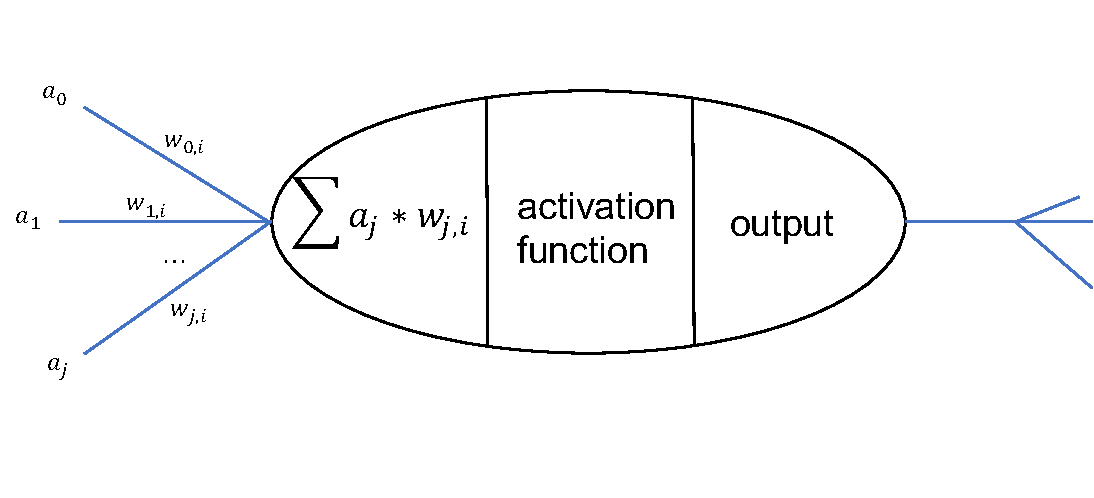
\includegraphics[width=1\linewidth]{neuron}
	\caption{Artificial neuron, according to McCulloch-Pitts neuron model \cite{McCulloch}.}
	\label{fig:neuron}
\end{figure}
A \gls{NN}, or an \gls{ANN}, is a metaheuristic that is inspired by nature, in that it mimics the general operation of a brain in a smaller scope. A neural network consists of multiple neurons that are connected with each other. Neurons are also called nodes and the connections are also called links and have an associated weight. In \autoref{fig:neuron} an artificial neuron, according to a McCulloch-Pitts neuron model \cite{McCulloch}, is visualised. Each neuron calculates the sum of its inputs, where the inputs may be the weighted outputs from other neurons if the neuron is on the hidden or output layer. If the neuron is on the input layer the inputs are usually unweighted. The output of each neuron located on the input and hidden layer are the input of the neurons that are located deeper into the NN. The output of neurons that are located on the output layer are depicted as the output of the whole NN.  The sum is the parameter for the activation function, usually a sigmoid function. \\
These networks, while being a rather simple construct, can implement every continuous function by using three layers (one hidden layer) and every function by using four layers (two hidden layers) \cite{russel}. \\
Neural networks are structured as depicted in \autoref{fig:nn}. The shown neural network is a feedforward NN, where no cycles are allowed. In this case the NN is stateless and does not implement memory, whereas a recurrent neural network (RNN) has directed cycles and states. A RNN exhibits dynamic temporal behaviour, whereas a feedforward NN can only react on the current inputs.
\begin{figure}[h]
	\center
	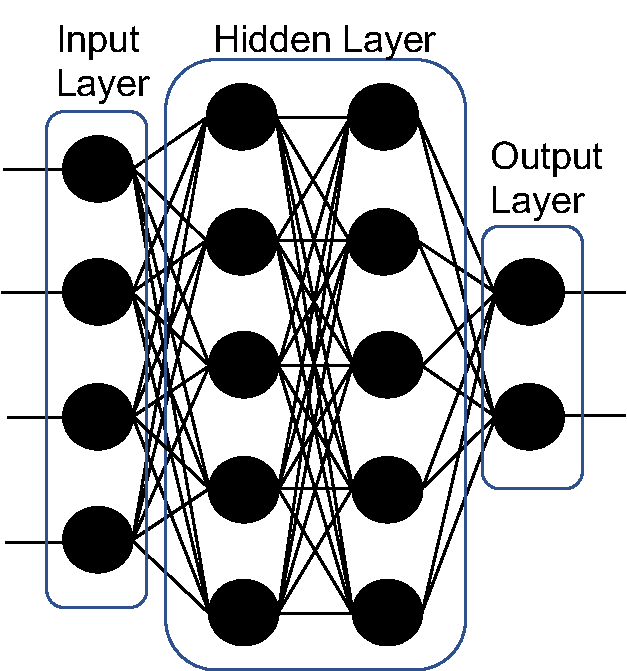
\includegraphics[width=0.7\linewidth]{nn}
	\caption{Neural network with hidden layers}
	\label{fig:nn}
\end{figure}

\section{Evolutionary Algorithms}\label{sec:evoalgo}
Evolutionary algorithms mimic evolution observed in nature. They are based on the simple principle: "survival of the fittest". Also the mechanisms of reproduction, mutation and selection are heavily inspired by nature. Basically all evolutionary algorithms follow these steps in an iterative manner. An iteration is called an epoch and the population of one epoch is a generation. Each generation consists of organisms, which are computer programs that have to solve the aimed problem. The computer programs are made up of simple code constructs named genes. For example, a neural network can be coded with its links and neurons as genes, like it is coded in NEAT.\\
To be able to know how well these organisms can solve the aimed problem, or to get to know how "fit" they are, a fitness function is needed. A fitness function should increase in value corresponding with the ability to solve the aimed problem.\\
One evolution is conducted as follows:
\begin{enumerate}
	\item{Create a random population.}
	\item{Calculate the fitness of the organisms in the population.}
	\item{Eliminate the worst performing organisms.}
	\item{Allow reproduction and mutation of the fittest organisms.}
	\item{Calculate the fitness of the organisms in the population.}
	\item{Check if the target fitness is achieved by any organism.}
	\item{If fitness is not achieved: Go to step 3. Else: Terminate.}
\end{enumerate}
\section{Mutations}\label{sec:mutation}
In NEAT \cite{neat} mutations can change link weights as well as structure, whereas in general genetic algorithms only the link weights are mutated in an evolution. This allows for evolving without prior structure to achieve results with minimal structure.
 There are four different mutations used in NEAT:  \emph{Link Weight Mutation},  \emph{Add Node},  \emph{Add Link} and  \emph{Switch Link}. \\\\
\textbf{Link Weight Mutation.} Simple mutation that changes the link weight randomly. \\\\
\textbf{Add Link.} Simple mutation that connects two nodes that are not already connected with each other. \\\\
\textbf{Switch Link.} This mutation randomly turns on or turns off a link. \\\\
\textbf{Add Node.} A node is placed between two already connected nodes. At first the connecting link is disabled and two new links are created. The node where the now disabled link was going out from is connected to the new node with weight 1. The new node is connected into the previous incoming node with the weight the now disabled link has. By doing this, the mutation has no immediate effect on the fitness of the neural network, depending on the activation function.

\section{Genetic Encoding}\label{sec:genenc}
The crucial point of NEAT is the genetic encoding. This genetic encoding allows NEAT to keep track of the history of evolved neural networks. Every gene has an innovation number, which are globally unique. If a mutation with the same effect happens, i.e. node~1 and node 3 get connected in two different neural networks, then both newly created genes have the same innovation number. These innovation numbers are needed for mating, described in \autoref{sec:mating}. \\
All information of a neural network is saved in genomes, also called genotypes. There all nodes and all connections are listed with their innovation numbers as well as their achieved fitness values. The genotype is not to be confused with the phenotype, where the neural network itself is saved. Between iterations, the worst performing members of a species, further explained in \autoref{sec:speciation}, get eliminated and thus make room for new organisms. 

\section{Mating}\label{sec:mating}
\begin{figure}[h]
	\centering
	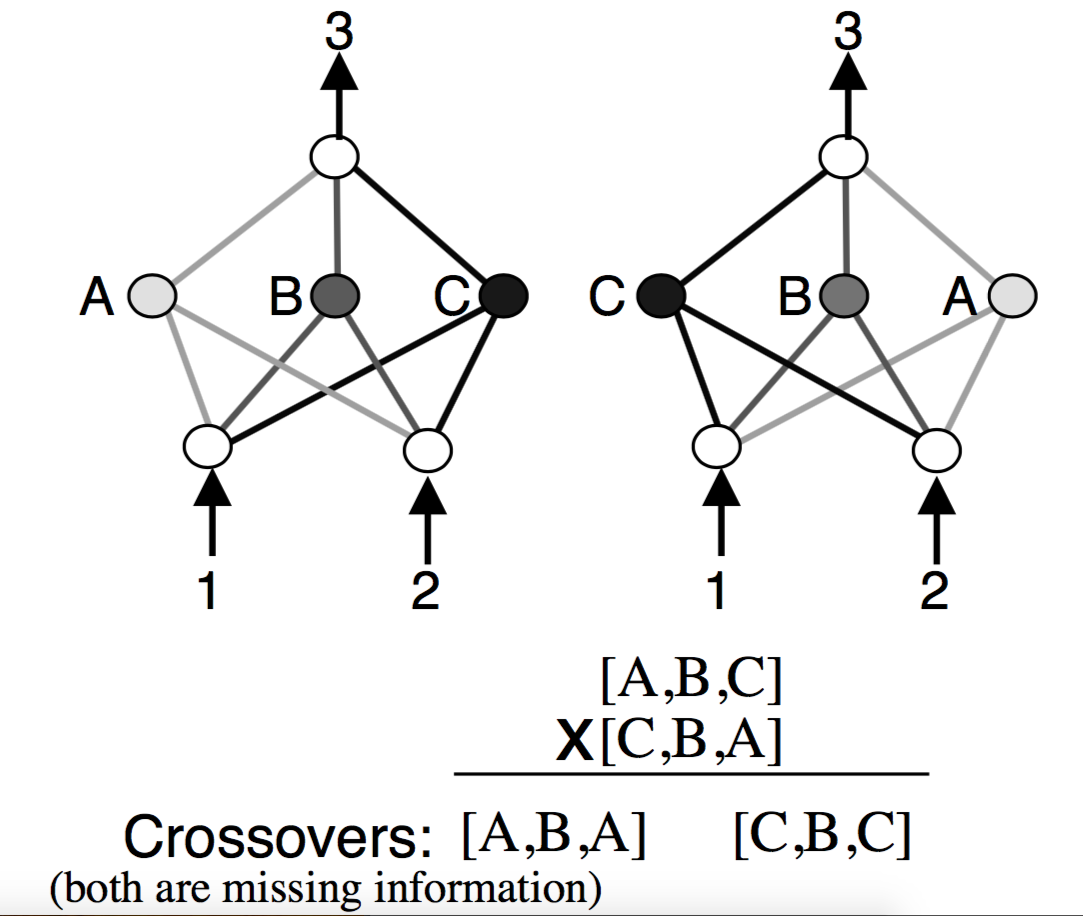
\includegraphics[width=0.7\linewidth]{competingConventions}
	\caption{Competing conventions}
	\small
	Even tough the two shown networks compute the exact same function, the ordering of its genes is different. When trying to crossover them, the resulting network is missing one of the 3 main components. This makes crossover pointless, because it would result in a random network instead of featuring the main components of both parents. \cite{neat}
	\label{fig:crossover}
\end{figure}
The prior explained genetic encoding is crucial for crossover operations in NEAT. With it, two genomes can be easily aligned and inspected for similarities and disparities. This solves the problem of competing conventions, where two networks compute the same function are chosen for crossover but are differently organised, visualised in \autoref{fig:competingConventions}.  \\

\begin{figure}[h]
	\centering
	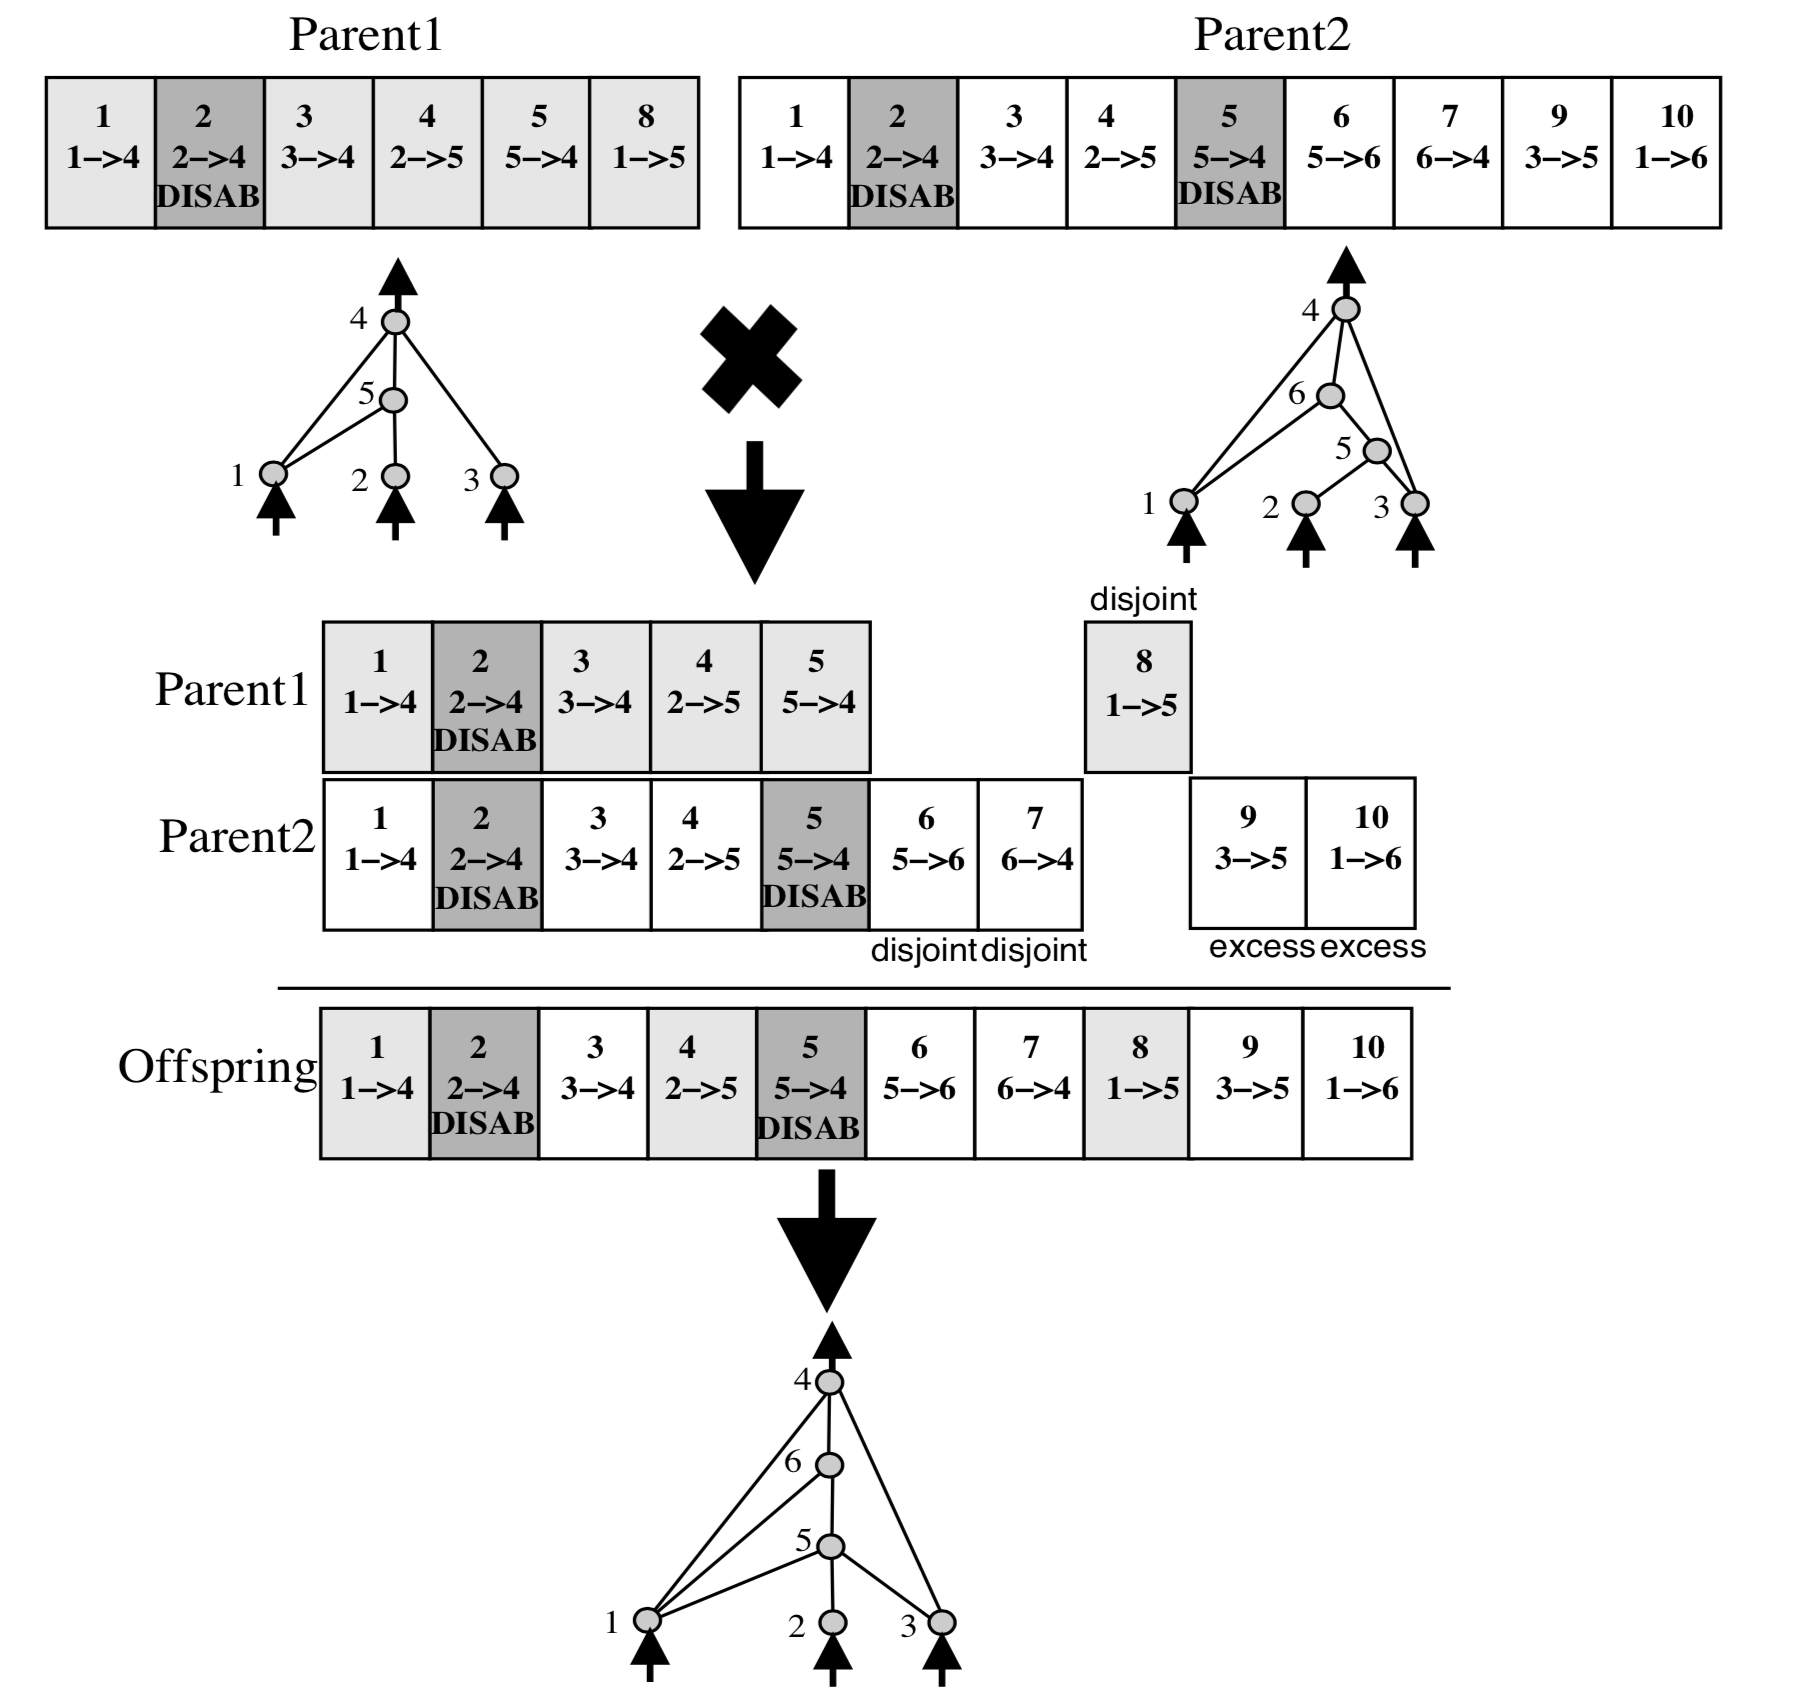
\includegraphics[width=0.9\linewidth]{mating}
	\caption{Visualisation of crossover from the NEAT paper \cite{neat}}
	
	\small
	 {Both parents share the same fitness, which is why disjoint genes are completely adopted.}
	\label{fig:crossover}
\end{figure}
In crossover, \autoref{fig:crossover}, the two genomes are compared with each other. For each gene, this can have three different outcomes. Either the genes match, then one of them is taken randomly into the new genome. The genes are disjoint, which means that one gene is present in one genome but not in the other and has a smaller innovation number than the maximum innovation number of the other genome. Then the disjoint genes of the fitter genome are adopted. Or the gene can be excess, which is when the gene has a higher innovation number than the maximum of the other genome. There also the ones from the fitter partner get adopted.

\section{Speciation}\label{sec:speciation}
One last characteristic of NEAT is speciation. Rather than having a single population of genomes competing against each other, NEAT splits it into species, forming smaller niches for neural networks to evolve rather isolated. This is done because neural networks after a mutation of structure are prone to have lower fitness, then slowly recover and maybe exceed the prior fitness. If there was no speciation, neural networks after a mutation of structure would just be thrown away to make room for "better" neural networks. To give them more time to evolve, neural networks with similar structure are bound together in a species and compete only against each other. This protects the innovation of these structures, that are endangered to be overtaken by other neural networks with less innovation but higher immediate fitness. \\\\
In each iteration, the population is split into species linearly, by taking a genome and calculating the compatibility distance to representatives of the species. This function takes the excess, disjoint and the average link weight differences of matching genes into account and weights them against each other. If it is below a compatibility threshold it will be put into that species. If there is no species where this holds a new species is created with this genome as a representative. Then, the worst performing members of each species are eliminated and replaced by the offspring of the remaining genomes. 





%*****************************************
\chapter{Related Work}\label{ch:relatedwork}
%*****************************************
\glsresetall % Resets all acronyms to not used

In this section, we look into related work in the field of (i) congestion control in wireless multi-hop networks, followed by (ii) techniques for data-driven generation of congestion control mechanisms. We also look into the usage of (iii) neural networks in communication networks and (iv) usages of NEAT in other fields.

\section{Congestion Control in Wireless Multi-Hop Networks}
\label{sec:rel_cong_control}
In wireless multi-hop networks, congestion control does not work the same way as in wired networks. In general, conventional congestion control interprets every packet loss as it being the result of congestion within the network. In wireless networks this assumption is not accurate, because packet loss can happen due to transmission errors or interferences. Also traditional congestion control relies on \gls{RTT} to update its congestion window. This is because it reacts on received ACKs and timeouts. In \gls{WMN}s, RTT can highly vary because of for example cross flows or mobility. \\ \\
Wireless Control Protocol (WCP) \cite{wcp} is a congestion control algorithm for wireless multi-hop networks, that addresses the head of line blocking effect, where a flow can not be served because it would interfere with other flows within the network. WCP does it by defining congestion as a neighbourhood phenomenon, happening at a link with all its reachable nodes within its transmission range, rather than at a single node. It also extends the TCP header with a congestion bit, which explicitly indicates that one link is congested. This bit is set by the node that registers congestion and distributes this information to all nodes that are in the region of that congested link which is up to a two hop range by setting this bit on all outgoing TCP packets. WCP uses \gls{AIMD}, like traditional TCP, but not on single nodes independently and rather simultaneously on all nodes, coordinated by the highest RTT within the network. \\
WCP improves the fairness in wireless multi-hop networks a lot, compared to other TCP flavours, which is the goal of this work. There are topologies where flows are starved when using TCP New Reno, for example. In \autoref{fig:wcpTopology}, flow 4 $  \rightarrow $ 6 is not served when using traditional TCP. But when using WCP, this flow is served and has about the same throughput as the others.
\begin{figure}[h]
	\centering
	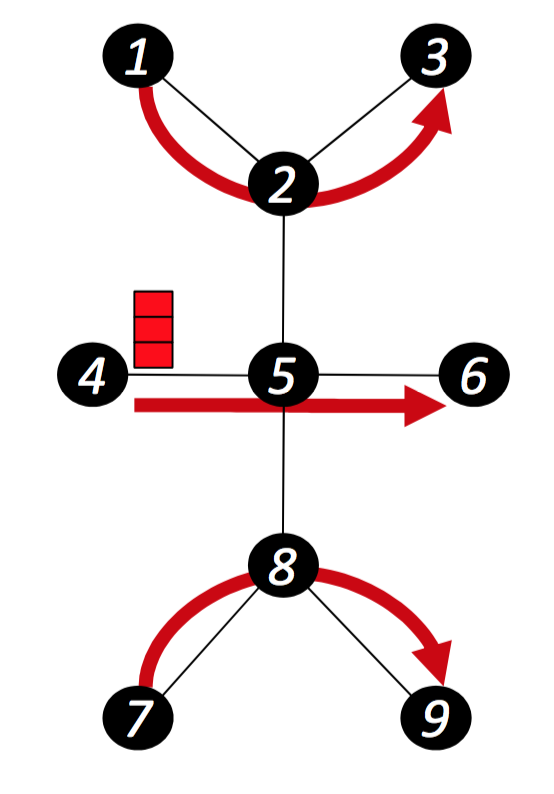
\includegraphics[width=0.45\linewidth]{wcpTopology}
	\caption{Wireless multi-hop network \cite{wcp}}
	\label{fig:wcpTopology}
\end{figure}
WCPCap extends WCP by also taking the collision probability at the receiver, the idle time perceived by the transmitter for each link and an estimation of link capacities at nodes into account for the decision process. This decision process neglects the capture effect and assumes that channel losses are known. WCPCap improves the fairness between flows even more than WCP.
\\\\ 
Intelligent TCP \cite{iTCP} or iTCP is a neural network based congestion control algorithm for wireless ad-hoc networks. It is a feed-forward neural network consisting of nine nodes with several different activation functions and three hidden layers,  that calculates the congestion window with the number of duplicate ACKs, number of timeouts and the last congestion window as parameters, as visualised in \autoref{fig:itcp}. Mobility is taken into account by not using parameters that would differ when the position is changed, like RTT. In this work, we use iTCP as a performance baseline, look at its implementation, port it from ns-2 to ns-3 as described in \autoref{sec:itcpimpl}, and discuss its performance in \autoref{ch:evaluation}.

\section{Learning Congestion Control}
\label{sec:rel_learning_networks}

Recent research has demonstrated innovative approaches to automatically generate congestion control mechanisms in computer programs rather than formulating their functioning manually. An innovative concept of learning congestion control is Remy \cite{remy}, which generates it by optimising offline simulations of the target network, rather than by evolution like in this work. Remy needs to know the target network as close to reality as possible so that the generated algorithm works on the real network. The generated congestion control algorithm is a simple reflex agent, meaning that it reacts on the current state of the network. The generation of a congestion control algorithm with Remy is a resource and time intensive task, since the network has to be simulated a lot of times. Remy generates a multidimensional rule-map, like in \autoref{fig:remy}, where the time between ACKs, the time between TCP sender timestamps and the ratio of current RTT to minimum RTT are mapped to an action on the congestion window. The generation starts with one rule and by splitting the most used rule within one simulation, the needed area of operation is refined by each iteration. The evaluation is done by calculating a utility function, that values the current rule-map. There it can be specified in which relation the congestion control algorithm has to be optimised. Multi-criteria optimisation is possible, like minimising delay and maximising throughput at the same time. 
\begin{figure}
	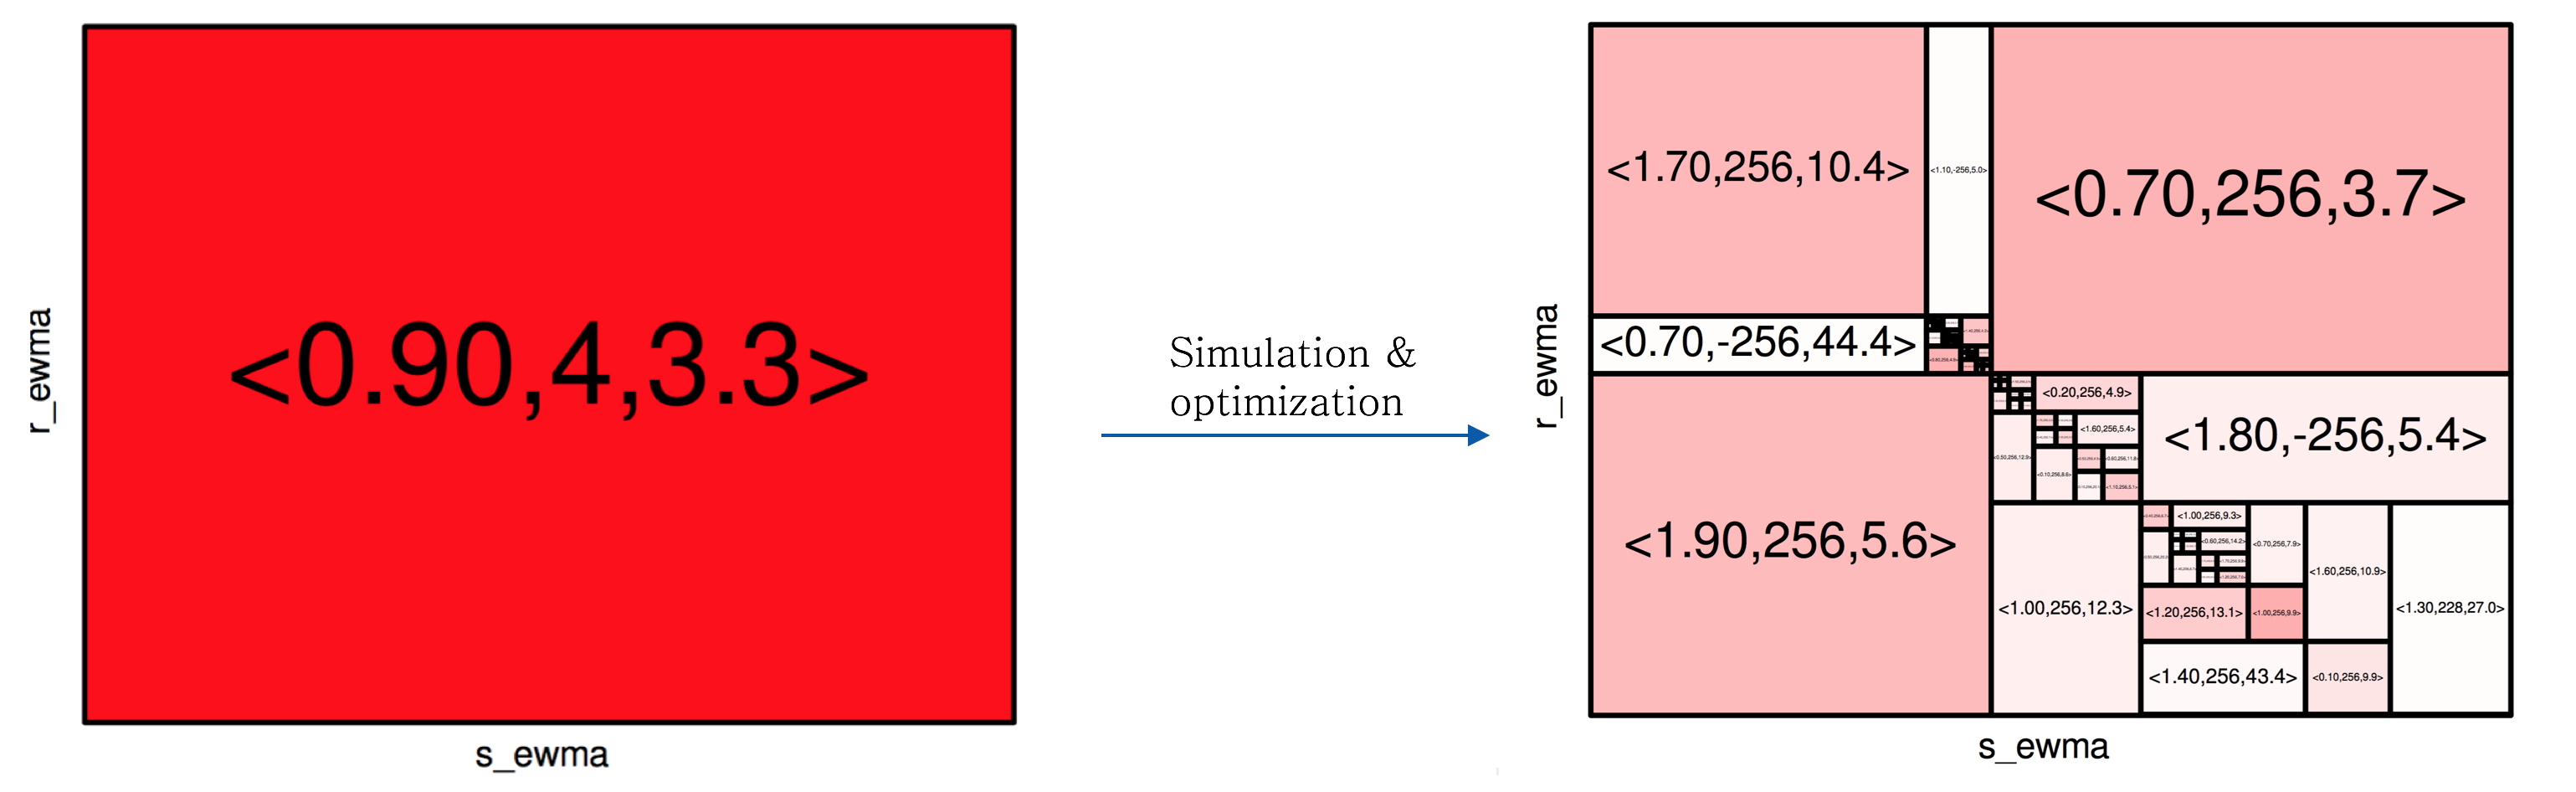
\includegraphics[width=1\linewidth]{remygraphic}
	\caption{Remy rule map, two dimensional \cite{remySlides}}
	\label{fig:remy}
\end{figure}
The problem with Remy is that it can be stuck in local maxima and has not been documented to work for wireless or wireless multi-hop networks. 
\\ \\
The authors of Remy published a follow up study on the general learnability of congestion control \cite{learnCC}. At first all of their results may not be applicable to wireless multi-hop networks. They state that there are network parameters that do not need to be exact and thus working for a range of these parameters qualitatively the same. For example, the network topology can be simplified. This may apply to wired networks but in our case with wireless multi-hop network, the network topology is one of the most influential characteristics. This is because if, for example, two nodes are communicating with each other, it would result in a different behaviour if there is a node in between them or not. In conclusion, learning a congestion control algorithm is possible and provides good results. However, learning a congestion control algorithm for a special network paradigm like wireless multi-hop networks has not been done in their work and thus the results of the prior mentioned papers should be taken with care.

\section{Neural Networks in Communication Networks}
\label{sec:rel_nn}
Neural networks have a wide range of usages and solve problems that are perceived as requiring intelligence, like face recognition in the new iPhone X. The use of neural networks is a promising approach of improving various facets of communication networks, which is further corroborated in this work. In this subsection, we look only into the use of neural networks in routing and handoff mechanisms. \\
Kojic et al. proposed a neural network based hybrid routing protocol for wireless mesh networks \cite{nnwmn}. Their idea was to use a Hopfield neural network because it can solve the traveling salesman problem. A lot of parameters are used: traffic load of each link, link delays, hop count and link capacities. The objective for the \gls{NN} is to find a path with as much free link capacity as possible. The output is a matrix of all links in the network, marked if used by the route. \\
This proposed routing \gls{NN} has been tested against \gls{AODV} and \gls{OSPF}. It outperformed these established routing protocols in terms of throughput, packet delivery ratio and blocking iterations. In the simulations, end-to-end delay was on par with the others, but proposed by the authors, that it would also outperform here, given the \gls{NN} is implemented on hardware, thus having better performance. 
\\\\
NNCH (Neural Network Based Context Aware Handoff) \cite{nnhandoff} makes use of neural networks to make the decision to handoff in wireless cellular networks. A handoff is the change of cells from a moving mobile device. If a mobile device is approaching the end of the zone of one cell, the device still wants to be connected, thus the nearby cell takes over the communication. The NN has to learn the cross-layer nonlinear correlation between packet success rate and link state indicators like \gls{SIR} and \gls{SNR}. In the paper it is shown that NNCH does surpress unnecessary handoffs. For example versus 0 dB \gls{THO} it reduces the number of handoffs by 96\%.


\section{Usages of NEAT in Other Fields}
\label{sec:rel_genalgo}
NEAT \cite{neat}, further explained in \autoref{ch:neatworking}, is used in a wide variety of fields, the most prominent being game playing with a video of MarI/O \cite{mario} \cite{marioneat}. A NEAT implementation in LUA evolving NNs that are able to get through the first level of Super Mario has millions of views on youtube. In \autoref{fig:mario} you can find a screenshot of that video. The fitness function in MarI/O simply is the travelled distance in direction to the end. There are some extensions of NEAT: real-time NEAT \cite{rtneat}, hyper NEAT \cite{hneat}, multi-agent hyper NEAT \cite{mahneat}, content-generating NEAT \cite{cgneat}, online/decentralised NEAT \cite{odneat}, NEAT fields \cite{neatfields} and Deep NEAT \cite{deepneat}, to name a few. \\
In the rest of this section some of the extensions are explained: \\
\begin{figure}
	\center
	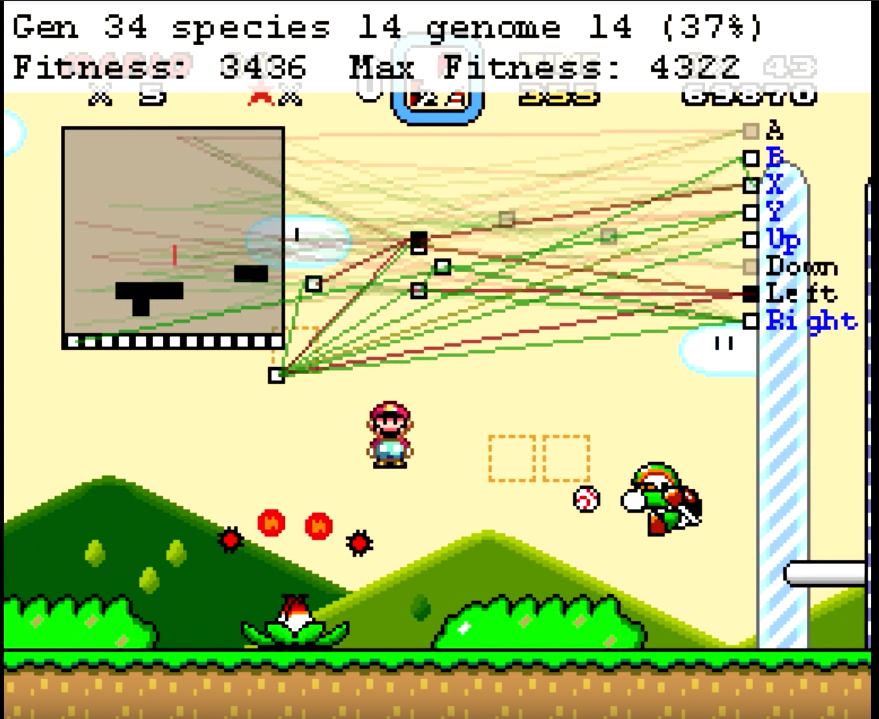
\includegraphics[width=0.8\linewidth]{mario}
	\caption{Screenshot of MarI/O \cite{mario}}
	\label{fig:mario}
\end{figure}
\textbf{cgNEAT} or content-generating NEAT \cite{cgneat} is used in a game called Galactic Arms Race \cite{gar}. There cgNEAT is used to generate new weapons based on usage statistics. It is not quite common for a game to generate its own new content. \\ \\
\textbf{rtNEAT} or real time NEAT \cite{rtneat} is an extension for evolving neural networks in real time. Originated from rtNeat is for example NeuroEvolving Robotic Operatives or NERO \cite{nero}. NERO is a video game where simulated robotic agents have to manage continuously changing environments and situations in fighting other players` robots. \\ \\
\textbf{NEAT fields} and \textbf{DeepNEAT} extend NEAT in such a way that it can cope with more input data as well as a high amount of hidden layers and number of neurons. NEAT fields \cite{neatfields} provide the possibility that a large number of input and output parameters can be used, without the performance collapse NEAT would have. DeepNEAT \cite{deepneat} extends NEAT with the possibility of using deep neural networks, also without the performance collapse NEAT would have. \\
\\
In this thesis the standard NEAT implementation is used because none of the extensions are expected to provide any positive effect. We only incorporate three parameters as inputs, so NEAT fields is not needed. Also congestion control is assumed to be a control problem, which NEAT is well capable of solving. For example, it can solve the double pole balancing problem even without velocity information which makes it non-Markovian \cite{neat}. Multi-agent NEAT, which performs a simultaneous evolution of multiple different agents, is not considered in this work, as we expect faster convergence when all nodes behave equally. Further investigation of multi-agent NEAT in the context of WMNs may be addressed by future work.

